
\begin{dialog}{对位藏头诗}

\begin{quote}
阿基里斯来拜访乌龟,看到乌龟家里有许多唱片。
\end{quote}

\begin{dialogue}

\item[阿基里斯]\rotatebox[origin=c]{180}{\emph{赫}}\CJKglue 赫有名的法国作曲家德彪西你知道吧?你这里有没有他的作品?

\item[乌龟]\emph{赫}赫有名的得镖器?我可没听说过。我这儿倒收藏了不少“飞去来器”,就是那种扔出去能飞回来的飞镖。

\item[阿基里斯]\emph{有}名极了,不过这没关系。你这里到底都有谁的作品?我想总该有巴赫的吧?

\item[乌龟]\emph{名}曲我都有,巴赫的自然不用说了。你听过巴赫的曲子吧?那种美,那种技巧!我每次听他的曲子都有新的感受。

\item[阿基里斯]\emph{的}确是技巧高超,百听不厌。哎,龟兄,你是从哪儿找来这些唱片的?

\item[乌龟]\emph{德}意志,巴赫的故乡。到底还是德国人演奏的好。

\item[阿基里斯]\emph{国}籍不重要,巴赫属于全世界。

\item[乌龟]\emph{作}为一种个人嗜好,我还是宁愿听德国人的演奏。好了,咱们别谈这些了,有句拉丁格言,恐怕你也知道:口味无须争辩。哎,你知道我这些天在干什么吗?我在研究一种特殊的音乐。这种音乐能形成一个“家族”,我称之为“粉碎唱机的音乐”。

\item[阿基里斯]\emph{曲}名就是这个?

\item[乌龟]\emph{家}族音乐是许多相似但又不同的曲子的总合,并没有什么总的曲名。我说的“粉碎唱机的音乐”不是曲名,而是对这一大族曲子的描述。

\item[阿基里斯]\emph{给}我讲讲是怎么回事吧,我现在一点也摸不着头脑。

\item[乌龟]\emph{了}解这种音乐可不是一件简单的事情,这得从头说起。有一次螃蟹来我这里做客,当时我身体不太舒服——噢,对了,你见过螃蟹吗?

\item[阿基里斯]\emph{我}没见过。不过已经久闻他的大名了,真希望能见到他。我本来应该有个机会能碰上他的,那是在一个叫凯瑟林的人家里。他家举办了一个音乐会,可我没能去成。我好像记得凯瑟林是个什么贵族,大概是个侯爵。

\item[乌龟]\emph{侯}爵,没错,就是后知后觉的那个侯爵。巴赫的《哥德堡变奏曲》就是为他写的。

\item[阿基里斯]\emph{世}上竟有这样不幸的事!这真太遗憾了,我不仅错过了螃蟹,还错过了那部著名的组曲!咳,我真是!

\item[乌龟]\emph{达}观一些,阿基。你将来肯定会有机会听《哥德堡变奏曲》,见螃蟹也是迟早的事,说不定哪天在公园里我们就会碰上他。别这么垂头丧气的。你平日的那股灵气呢?

\item[阿基里斯]\emph{灵}气?好吧,你接着说吧:螃蟹到你这儿来了,当时你不大对劲——

\item[乌龟]\emph{感}到身体不太舒服,也正想找人聊聊,于是他跟我说起他新买的唱机——你知道,螃蟹这家伙特别容易对小玩艺着迷,这回轮到唱机了——他说他那唱机是一台完备的唱机,能重现任何音乐。我当然不信,可我没法说服他。他顽固地相信推销员对他说的每一个字!于是我回家后研究了一番,作了一支曲子,灌进唱片,带着去见螃蟹。这支曲子的名字是“我不能在唱机1上播放”,就是说……

\item[阿基里斯]……什么?那是个什么东西?

\item[乌龟]\emph{在}唱机1上没法播放的曲子,就是这么回事。我建议他听听这支曲子,他很高兴地答应了,把唱片放上那个可爱的唱机。可是真不幸!刚刚播出几个音符,那唱机就开始剧烈地震颤起来,随后“砰”的一声巨响,唱机炸成了碎片,溅得满屋都是。唱片当然也跟着完了。

\item[阿基里斯]\emph{此}刻螃蟹一定非常难受吧?你也太狠心了!

\item[乌龟]\emph{我}不过是向他证明一下他的观念有多么荒唐罢了。那台唱机根本不可能重现我那支曲子,那种音乐会使它震碎自己。

\item[阿基里斯]\emph{借}用一个术语,就是“自我震碎”了,对吗?

\item[乌龟]\emph{用}得好!当然,也可以这么看这个问题:那个推销员多少有些吹牛,螃蟹买的那台唱机不是那么完备,它事实上不可能重现所有的音乐。

\item[阿基里斯]\emph{他}后来明白这一点了吗?我想他不会就此罢休吧?

\item[乌龟]\emph{的}确,他没认输,他后来……嗯,我想我该先讲讲我的曲子,是不是?

\item[阿基里斯]\emph{对}对,你应该先跟我说说你的曲子是怎么回事。等一下,那种唱片你只有一张吗?我很想看看。你把它放在哪儿啦?

\item[乌龟]\emph{位}子上。在那儿。\dlnote{(阿基里斯找到了唱片。)}看唱片是看不出什么的,关键在于曲子的旋律。唱机播放这种旋律时会产生特殊的音响效果。我可以给你详细讲讲。在回访螃蟹之前,我去了螃蟹买唱机的那家商店,问清了制造那种唱机的工厂。然后我给制造商写了一封信,向他们索取设计图纸。得到图纸以后,我仔细分析了那种唱机的结构,发现只要附近有某种特殊的声音,就会引起唱机的共振,最终导致它破碎。

\item[阿基里斯]\emph{技}术方面的问题你倒挺在行的。

\item[乌龟]\emph{巧}妙地把这种声音组织成旋律,就是那首“我不能在唱机1上播放。”

\item[阿基里斯]\emph{写}上“礼物”二字,送给螃蟹,这就是你干的好事!螃蟹真是太不幸了。后来呢?

\item[乌龟]\emph{下}一次我见到他时,他说他又买了一台新的唱机。他不认输,他无论如何不相信那是唱机的问题。这台新唱机比上一台贵得多,推销员保证说如果发现有什么音乐那唱机无法重现,就付还他双倍的钱。螃蟹跟我说这些的时候兴高采烈,我答应了去看看他的唱机。

\item[阿基里斯]\emph{一}定又是这么个过程:在你去之前,你写了一封信给制造商。然后你针对这个唱机的结构谱一支曲子,叫做“我不能在唱机2上播放”,到了螃蟹那儿以后,同样的事情发生了,唱机炸成了碎片,唱片也毁了。对不对?

\item[乌龟]\emph{个}别时候你倒也挺聪明!你说的完全正确。看来你已经抓住了这件事的核心。

\item[阿基里斯]\emph{对}我来说这不算什么。我要是螃蟹,早就看穿你这一套了,根本不会让你钻空子。我会设计一个能对付你这花招的唱机。唉!只可惜螃蟹想不到这一点。

\item[乌龟]\emph{话}可不能这么说。我和螃蟹又较量了几个回合之后,他也明白了我的手段。于是他变得聪明了,准备……

\item[阿基里斯]\emph{并}不是螃蟹聪明。你那手段本来就没什么了不起的。螃蟹可以很容易就战胜你:比如说用一台低保真的唱机——无法严格重现那种能够毁坏自己的声音——你不就没辙了?

\item[乌龟]\emph{嵌}上一块亮晶晶的小牌子,标明它是个“完备”的唱机,对吗?你怎么这么糊涂!一开始就确定了有些音乐不能重现,还算什么完备的唱机?你想想……

\item[阿基里斯]\emph{进}一步的解释让我来作:如果一个唱机——就说是唱机X吧——有足够的高保真度,那么当它试图播放曲子“我不能在唱机X上播放”时,恰恰就引起了那种粉碎它自己的共振……所以它不是完备的。然而唯一能绕开这种打击的方法——即让唱机X是低保真的——却更直接地表明了它的不完备。看来任何唱机都会有这样或那样的弱点,因此所有的唱机都是有缺陷的。可怜的螃蟹,无论是高保真唱机还是低保真唱机,他都是注定要失败的。

\item[乌龟]\emph{他}的问题不在于使用了什么“有缺陷”的唱机。我不认为谈论唱机的“缺陷”有什么意义,一台唱机本来就不可能做你希望它做的所有事情。如果一定要说什么地方有缺陷,那也不是唱机,而是你对它们的期望——对于唱机能做些什么事情的期望。螃蟹恰恰就是充满了这类不现实的期望。

\item[阿基里斯]\emph{的}确,不应该责怪唱机。我估计螃蟹买的也一定是好唱机,名牌的。

\item[乌龟]\emph{名}牌不名牌无关紧要,反正是高保真的,因此注定要破碎。不过,螃蟹还是没认输。他知道了我谱曲的原理之后,想出了一个办法,他以为这样就能胜过我了。他写了封信给唱机制造商,描述了他自己发明的一种装置,让他们依法制造。螃蟹称之为“唱机欧米伽”。这是一种比一般唱机都复杂得多的唱机,复杂得以至于……怎么说呢?以至于……

\item[阿基里斯]\emph{字}斟句酌的干嘛?你就接着说吧,是什么样的?

\item[乌龟]\emph{以}至于我似乎真的没办法了。唱机欧米伽和一般的唱机有很大区别,但表面上差不多。

\item[阿基里斯]\emph{表}面上差不多但又有很大区别?那么就是内部构造很不一样了?给我详细讲讲吧,最好画个图。

\item[乌龟]\emph{示}意图是这样。\dlnote{(画了一个图,用笔指点着)}这是一部摄像机,连接着一台超微型计算机,都是嵌在唱机内部的,从外面看不出来。摄像机的任务是在播放一张唱片之前扫描其纹道,而计算机的任务是根据摄像机搜集的信息进行某种计算,精确地确定出这张唱片播放时会产生什么样的音响效果,判断它是否对欧米伽的唱机部分有害。

\item[阿基里斯]\emph{我}想象不出判断出有害了又能怎么样。

\item[乌龟]\emph{对}于那些有害的唱片,欧米伽自有一套聪明的办法。它有一个特殊的装置,能重新组织它的唱机部分,从而改变唱机的结构,使之播放那种唱片时不产生共振。这一切都在计算机的指挥下进行,精确可靠,因此任何一张唱片它都能播放——它总能选择一种不会产生共振的结构来播放一张唱片。

\item[阿基里斯]\emph{他}可真有两下子!

\item[乌龟]\emph{卓}绝的设计,是吧?

\item[阿基里斯]\emph{越}来越邪乎了,这个老螃蟹!你彻底失败了吧,龟兄?

\item[乌龟]\emph{才}没有呢!你恐怕不很了解哥德尔不完全性定理吧?按照这个定理,螃蟹再怎么耍花招也赢不了。

\item[阿基里斯]\emph{能}赢!我不知道什么“疙瘩”不“疙瘩”,反正你肯定输了。嗯,这个关于“粉碎唱机的音乐”的小故事还真挺有意思。好了,你也不用再讲下去了,事情的结局是非常明显的:你老老实实认输,即便你是那么不愿意——这由不得你!

\item[乌龟]\emph{由}不得我?\dlnote{(打了一个呵欠)}算了算了,今天算了,你瞧,已经快半夜了,我得睡觉了,下次我再跟你说都是怎么回事吧。

\item[阿基里斯]\emph{衷}心地感谢你。你的故事使我今天晚上很愉快。好,我回去了。\dlnote{(刚走到门边,忽然停下来转回身)}我真糊涂!差点忘了。这是一个小小的礼物,我特地带给你的。\dlnote{(递给乌龟一个整整齐齐的小包。乌龟打开一看,是一只高脚杯)}怎么样,不错吧?

\item[乌龟]\emph{的}确好极了!多么奇特的一只高脚杯!哎,阿基,你知不知道,高脚杯这玩艺儿还是挺让我着迷的。只是近来景况不佳……

\item[阿基里斯]\emph{景}况不佳?我不明白。

\item[乌龟]\emph{仰}头看看,那儿。\dlnote{(阿基里斯仰起头,看见一个架子上摆了一排高脚杯。)}我收藏了这么多高脚杯,可它们总是有这样那样的缺陷。我可以告诉你我的心愿,不过你得为我保密。我一直试图找一只完备的高脚杯:它的形状必须没有任何缺陷。但我始终没能如愿。如果你送给我的这只高脚杯正是我要找的,那岂不是太妙了?告诉我,阿基,你怎么搞到它的?

\item[阿基里斯]\emph{大}概不能告诉你,我很抱歉。这是我的一个小秘密。不过你应该知道这个高脚杯是属于谁的。

\item[乌龟]\emph{家}里有这么多高脚杯,我不可能一一知道它们的来历,当然,这只高脚杯我就更不知道了。还是你来告诉我吧。

\item[阿基里斯]\emph{也}好。它属于你最喜欢的作曲家巴赫。他有许多高脚杯,这一点不太为人所知——我给你的这个是他的最后一只高脚杯。

\item[乌龟]\emph{许}多高脚杯中的最后一只,是吗?我的天!如果这真是巴赫的,那将是无价之宝了。可你怎么能肯定这是巴赫的?

\item[阿基里斯]\emph{都}在上面写着呢。你看见刻在杯子上的那些精巧的字母了没有?

\item[乌龟]\emph{记}载着巴赫的名字!这只高脚杯的确是巴赫的,多不寻常啊!\dlnote{(小心翼翼地把这只高脚杯放在了架子上。)}哎,阿基,你知不知道巴赫的名字,也就是B-A-C-H,每个字母各是一个音名?

\item[阿基里斯]\emph{得}排除H。你知道,音名只是从A到G。

\item[乌龟]\emph{他}的情况有些特殊,你知道他是德国人,在德国,音名的记法和我们略有不同。我们用B的地方,他们用H,而我们用降B的地方,他们用B。比如说,我们说巴赫的“B小调弥撒曲”,他们却说“H小调弥撒曲”。明白了吗?

\item[阿基里斯]\emph{曾}经有人告诉过我这些,我怎么给忘了。现在我想起来了。这么说,巴赫的名字实际上是一段旋律喽?

\item[乌龟]\emph{把}那四个音符连续奏出,的的确确就是一段旋律。事实上,巴赫把这段旋律用意微妙地写进了他精雕细琢的一部作品——即《赋格的艺术》中最后一支四声部三重赋格里。这支曲子是巴赫所写的最后一支赋格。我第一次听它时,全然不知它会如何结尾。可突然,没有任何先兆,曲子戛然而止。然后……死一般的寂静。我立刻体会到巴赫就是在这儿死去的。那是一个难以名状的悲伤时刻,我的心都——碎了……B-A-C-H是那部赋格的最后主题,它隐藏在这支曲子里。虽然巴赫没有明白地表明这一点,但如果你知道这支曲子是怎么回事,你就会很容易发现了。

\begin{figure}
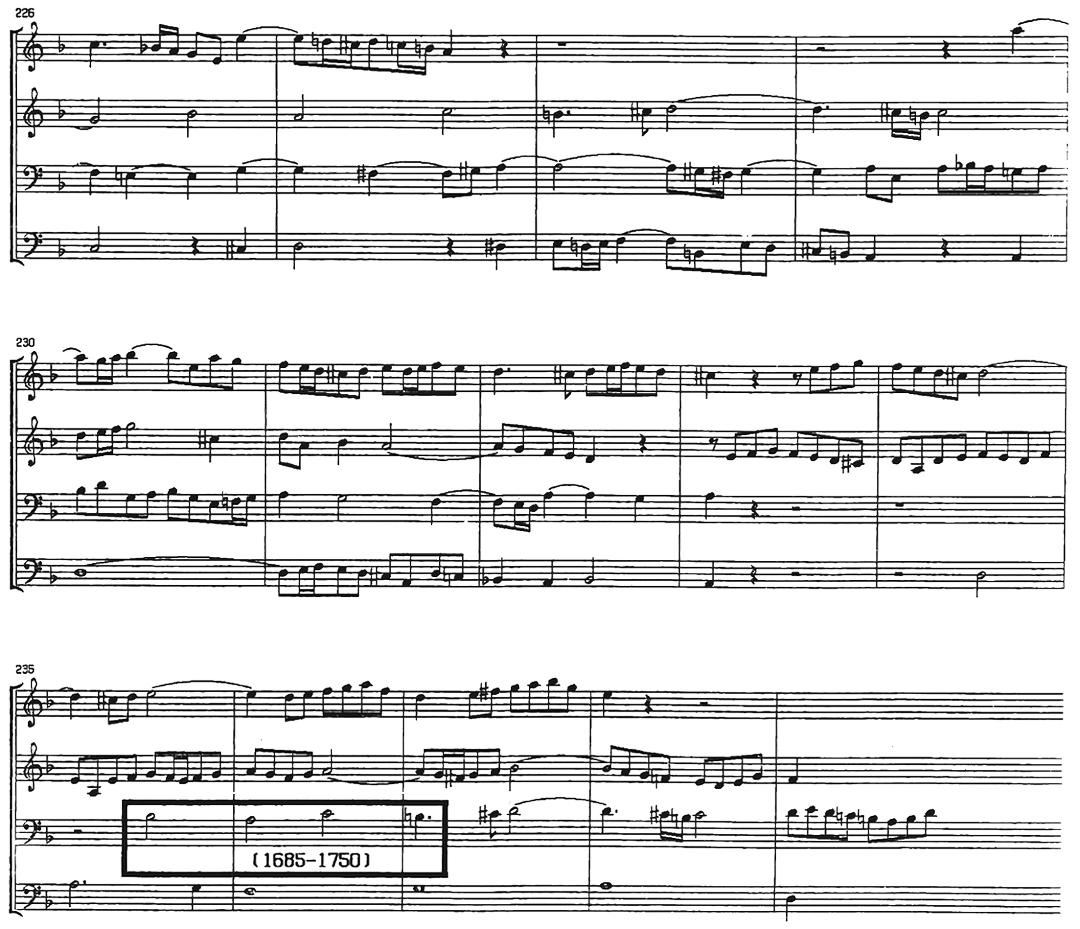
\includegraphics{img_019.png}
\caption[巴赫《赋格的艺术》的最后一页。]
  {巴赫《赋格的艺术》最后一页。在原手稿上,巴赫的儿子卡尔·菲利普·埃玛努厄尔写道:“请注意,在这支赋格中,当名字B. A. C. H.作为对题被引入时,作者死去了”(方框标出的即是B-A-C-H。)我把巴赫的这最后一支赋格的最后一页当作他的墓志铭。[乐谱由唐纳德·伯德的程序“斯马特”印出.该程序是在印第安纳大学开发的。]}
\end{figure}

\item[阿基里斯]\emph{他}为什么要那样呢?

\item[乌龟]\emph{的}确是个谜。无论如何,这是部杰作,而那段旋律也成为名句了。

\item[阿基里斯]\emph{名}句?有这么说的吗?

\item[乌龟]\emph{字}眼不重要,我相信你明白我的意思。

\item[阿基里斯]\emph{写}下来的精彩句子才称作“名句”,那是文学领域的事,你可别乱用。

\item[乌龟]\emph{进}入到文学领域你会发现更多这样的手法。比如说在刘易斯·卡罗尔的诗中,就常常把一些词或名字藏在每行的第一个字里。用这种方式藏有信息的诗称作“藏头诗”。

\item[阿基里斯]\emph{一}提起卡罗尔,我就会想起一个一直困扰我的问题:他是靠什么搞出了那么多妙不可言的玩艺儿?小时候我读过他的“炸脖\textcombine{卧龙}”,真是太绝了!

\item[乌龟]\emph{首}先是靠他的天才,我看是这样。这个我们先不管它,总之卡罗尔写过不少藏头诗。巴赫偶尔也写一点藏头诗,这并不奇怪。毕竟,赋格与藏头诗都同时有好几层隐藏着的意思,在这一点上两者颇为相似。多数的藏头诗只有一层隐含的意思,但是没有理由不让你搞出个双层结构——一首藏头诗中的藏头诗,或者也可以搞一个“头尾反藏诗”——把一句话最后一个字和第一个字连起来时,是一个有意义的词。天哪!形式本身具有的可能性几乎是无限的!赋格里就充满了这种技巧。

\item[阿基里斯]\emph{赋}格的情况更为复杂,是吧?

\item[乌龟]\emph{格}式更为多样,技巧要求更高。其实即使是写对话也可以使用这种技巧……嗯,我忽然有了个想法。你设想一下,一位对话作者为了表示他对巴赫卓越才能由衷的景仰而写下一篇对话,对于这位作者来说这样做是不是更合适:即在对话中借用巴赫的对位技巧嵌进自己的名字——或者巴赫的名字?咳,何必操那份心呢,谁愿意写这样一篇对话就写去吧。我们还是来看看巴赫那个作为旋律的名字吧。你知不知道,B-A-C-H这个旋律如果上下颠倒地从后向前演奏,会和原先正着演奏时完全一样?

\item[阿基里斯]\emph{曲}调怎么能上下颠倒演奏?从后向前我倒知道怎么回事——就是H-C-A-B——可上下颠倒会是什么样?你一定是在跟我开玩笑。

\item[乌龟]\emph{的}确能颠倒着演奏,真的。用颠倒的方式演奏尾声正合适。

\item[阿基里斯]\emph{尾}声怎么就合适?你能马上给我表演一下吗?

\item[乌龟]\rotatebox[origin=c]{180}{\emph{巴}}\CJKglue 不得呢。你等一下,我去拿小提琴——\dlnote{(走入另一个房间,不一会,拿着一把古雅的小提琴回来了)}——现在我来把这一段从前向后,从后向前以各种方式给你演奏一下,听好啊……

\bigskip

\begin{quote}
乌龟从架子上取下那只高脚杯,恭恭敬敬地把它倒置在谱架上,开始演奏B-A-C-,当他拉到最后一个音符H时,突然,没有任何先兆,高脚杯炸成了碎片,飞溅到乌龟跟前的地板上。然后……死一般的寂静。
\end{quote}

\end{dialogue}

\end{dialog}
